\subsubsection*{Maximum flow with minimum capacities}
%\url{https://atcoder.jp/contests/abc285/editorial/5535}

On the resulting graph, 
accumulate maximum flow in the following order:
\begin{itemize}
\item from $S'$ to $T'$
\item from $S'$ to $T$
\item from $S$ to $T'$
\item from $S$ to $T$.
\end{itemize}

An $S-T$ flow that satisfies the minimum capacities 
exists if and only if, for all outgoing edges 
from $S'$ and incoming edges to $T'$, 
the flow and capacity are equal.

\begin{center}
    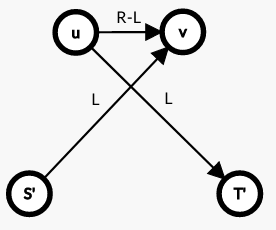
\includegraphics[width=0.1\textwidth]{content/graphs/max-flow-min-capacities.png}
\end{center}
